\documentclass[a4paper, 12pt]{article}

% basic text stuff
\usepackage[utf8]{inputenc}
\usepackage[T1]{fontenc}

\usepackage{tikz} % main tikz package
\usetikzlibrary{intersections} % to name paths and compute intersections
\usetikzlibrary{angles,quotes} % to plot and name angles

\definecolor{nblue}{rgb}{0.38, 0.51, 0.71} %glaucous, 97,130,181, #6182B5
\definecolor{nred}{RGB}{175, 49, 39} % AF3127
\definecolor{norange}{RGB}{217, 156, 55} % D99C37
\definecolor{ncyan}{RGB}{120, 169, 170}

\begin{document}

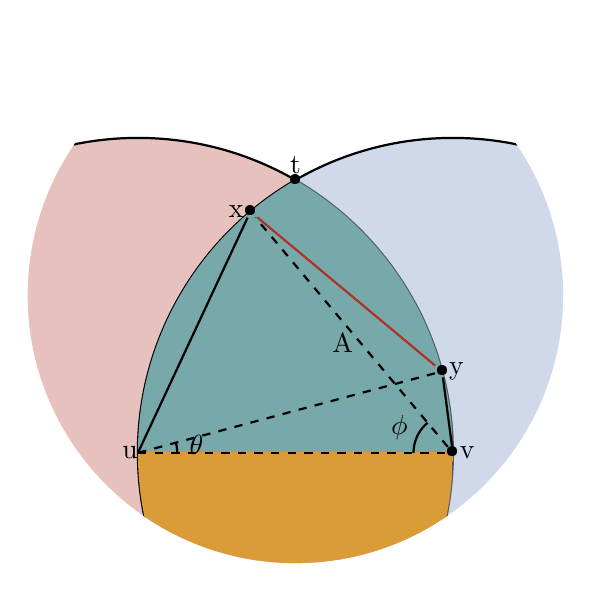
\begin{tikzpicture}[scale=2,thick]
    \tikzstyle{every node}=[minimum size=0.2,inner sep=0,outer sep=0]
    \clip (1,1) circle (1.7cm);
    \draw [fill=nred!60, fill opacity=0.5, name path=c1] (0,0) circle (2cm);
    \draw [fill=nblue!60, fill opacity=0.5, name path=c2] (2cm,0) circle (2cm);
    \begin{scope}
        \clip (0,0) circle (2cm);
        \clip (0,0) rectangle (2,2);
        \fill[ncyan] (2,0) circle (2cm);
    \end{scope}
    \begin{scope}
        \clip (0,0) circle (2cm);
        \clip (0,0) rectangle (2,-2);
        \fill[norange] (2,0) circle (2cm);
    \end{scope}
    \node[label=left:u] (u) at (0,0) {};
    \node[label=right:v] (v) at (2,0) {\textbullet};
    \begin{scope}[xshift=2cm]
        \node[label=left:x] (x) at (130 : 2) {\textbullet};
    \end{scope}
    \begin{scope}[xshift=0cm]
        \node[label=right:y] (y) at (15 : 2) {\textbullet};
    \end{scope}
    \draw (x) -- (y) [nred,>=latex];
    \draw (x) -- (u) [>=latex];
    \draw (y) -- (v) [>=latex];
    \draw (u) -- (y) [dashed,>=latex];
    \draw (v) -- (x) [dashed,>=latex];
    \pic [draw, -, "$\theta$", angle eccentricity=1.5] {angle = v--u--y};
    \pic [draw, -, "$\phi$", angle eccentricity=1.5] {angle = x--v--u};
    %\node[label={[label distance=0.2]-45:m}] (m) at (1,0) {\textbullet};
    \node (A) at (1.3,0.7) {A};
    %\node (B) at (0.7,-0.7) {B};
    
    \path [name intersections={of=c1 and c2,by=t}];
    \node[label=above:t] at (t) {\textbullet} ;
    \draw (u) -- (v) [dashed];
    %\draw (m) -- (t) [->,>=latex];
\end{tikzpicture}

\end{document}
